\documentclass[a4paper, 12pt]{article}
\usepackage[T2A]{fontenc}
\usepackage[utf8]{inputenc}
\usepackage[english,russian]{babel}
\usepackage{amsmath, amsfonts, amssymb, amsthm, mathtools, misccorr, indentfirst, multirow}
\usepackage{wrapfig}
\usepackage{graphicx}
\usepackage{subfig}
\usepackage{adjustbox}
\usepackage{pgfplots}
\usepackage{mathrsfs}
\usepackage{float}
\usepackage{geometry}
\geometry{top=20mm}
\geometry{bottom=20mm}
\geometry{left=20mm}
\geometry{right=20mm}

\begin{document}
\begin{titlepage}
	\centering
	\vspace{5cm}
	{\scshape\LARGE Московский физико-технический институт \par}
	\vspace{4cm}
	{\scshape\Large Лабораторная работа 16 \par}
	\vspace{1cm}
	{\huge\bfseries Изучение характериографа и методов визуального наблюдения и измерения статических характеристик полупроводниковых приборов \par}
	\vspace{1cm}
	\vfill
\begin{flushright}
	{\large выполнил студент группы Б04-005}\par
	\vspace{0.3cm}
	Смирнов Даниил
\end{flushright}

	\vfill
	
% Bottom of the page
	Долгопрудный, 2023 г.
\end{titlepage}
	
 \paragraph*{Цель работы:} ознакомиться с методами измерения статических характеристик полупроводниковых приборов и элементов ЭВМ с помощью характериографа. Измерить ВАХ полупроводниковых диодов.
	
\section*{Теория}

\textit{Полупроводники} – материалы, проводимость которого существенно зависит от примесей, температуры и других внешних факторов.

\textit{Диод} – двухэлектродный электронный прибор, обладающий нелинейной вольт-амперной характеристикой. Электрод диода, подключённый к положительному полюсу источника тока,
когда диод открыт (то есть имеет маленькое сопротивление), называют
анодом, подключённый к отрицательному полюсу — катодом.

\subsection*{Электронные уровни и переходы}

Наличие примесей в аморфных полупроводниках практически не дает вклада в проводимость, поэтому далее будут рассматриваться только полупроводники с кристаллической структурой.

Рассматриваем каждый атом решетки как потенциальную яму. При их сближении вероятность электрона протуннелировать в соседнюю начинает повышаться, при этом суммарная волновая функция может быть как симметричной, так и антисимметричной, что дает 2 различных энергетических уровня. В случае N атомов будет N энергетических уровней, что дает практически непрерывный спектр возможных значений энергии для электронов - такой подход называется зонной теорией. Все описанное ведет к появлению разрешенных и запрещенных значений энергии. С таким подходом можно определить понятие полупроводника, металла и изолятора: У металла при T=0 есть электроны в зоне проводимости (первой не заполненной зоне), у полупроводников и изоляторов - нет. При этом считается, что у полупроводников ширина запрещенной зоны (между первой незаполненной и последней заполненной (валентной)) от 1 до 3 эВ (рис. \ref{fig:theor_pic_0})

\subsection*{Механизмы электропроводности примесных полупроводников}

В кристаллических полупроводниках реализуется 2 типа проводимости: собственная и примесная.

\textit{Собственная проводимость} реализуется в результате ионизации атомов, однако такой тип дает существенно меньший вклад чем \textit{примесная проводимость}: часть атомов в решетке, в которой все электроны учавствуют в связях, заменяют на атомы с избыточным (например, атом мышьяка с 5 валентными электронами в решетке кремния с 4) или недостаточным (например, атом индия с 3 валентными электронами в решетке кремния с 4) числом электронов для образования связей, в результате чего в системе появляются лишние, ни с чем не связанные электроны или их недостаток (дырки). Такие полупроводники называются n-типом в случае электронной проводимости, а примесные уровни, обеспечивающие это - \textit{донорные} или p-типом в случае дырочной, а уровни - \textit{акцепторные}.

\begin{figure}[H]
    \centering
    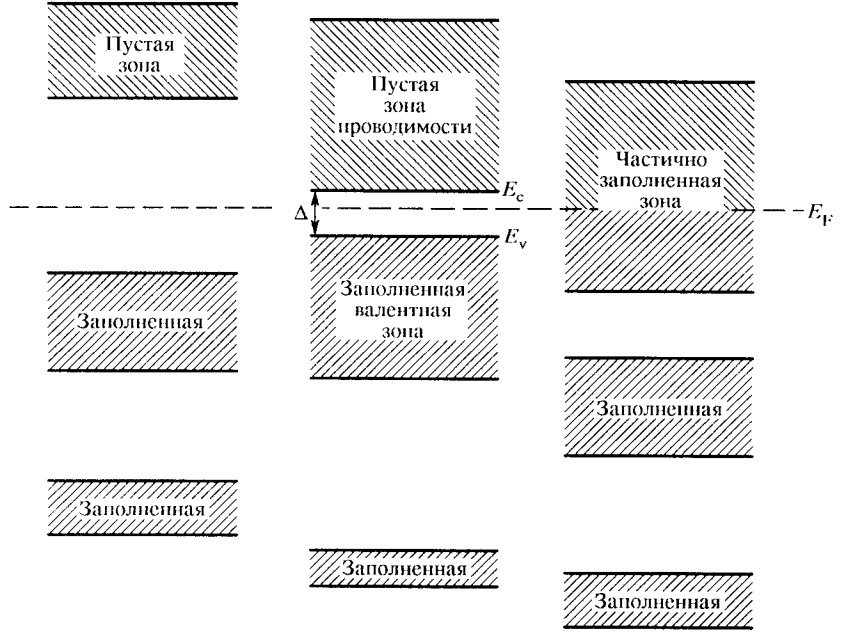
\includegraphics[width=0.7\linewidth]{Theor_pic_0.png}
    \caption{Энергетические зоны для а) изолятора б) полупроводника в) металла }
    \label{fig:theor_pic_0}
\end{figure}

\begin{figure}[H]
    \centering
    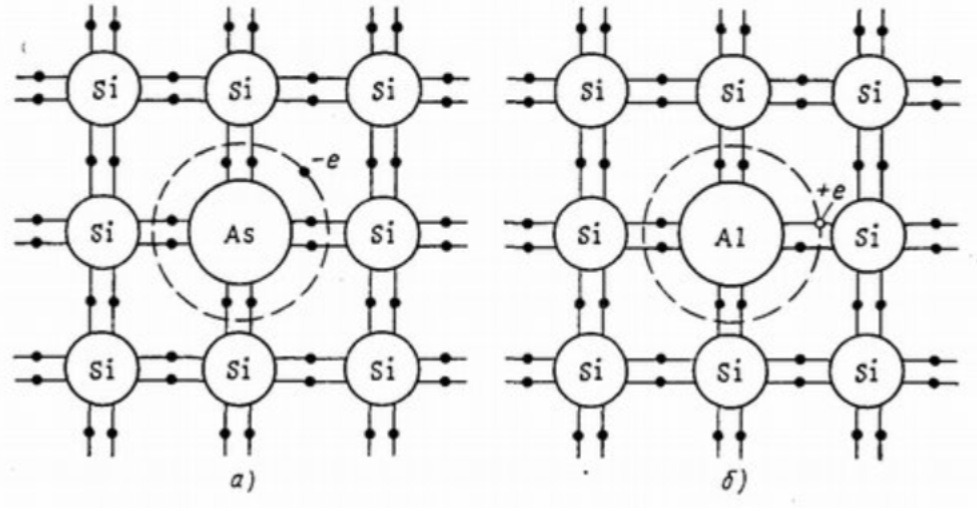
\includegraphics[width=0.7\linewidth]{Theor_pic_1.png}
    \caption{Двумерное представление расположения связей в решетке донорного (а) и акцепторного (б) полупроводников.}
    \label{fig:theor_pic_1}
\end{figure}
 
Наличие примеси в кристалле полупроводника будет характеризоваться появлением локальных уровней, лежащих в запрещенной зоне. Так при ионизации атома мышьяка образуется свободный электрон и для его возникновения требуется меньшая энергия чем для разрыва ковалентной связи кремния, энергетический уровень донорной примеси $E_d$ должен располагаться в запрещенной зоне близко к краю зоны проводимости. Акцепторная примесь имеет в запрещенной зоне уровень $E_a$, расположенный на небольшом расстоянии над потолком валентной зоны.

\begin{figure}[H]
    \centering
    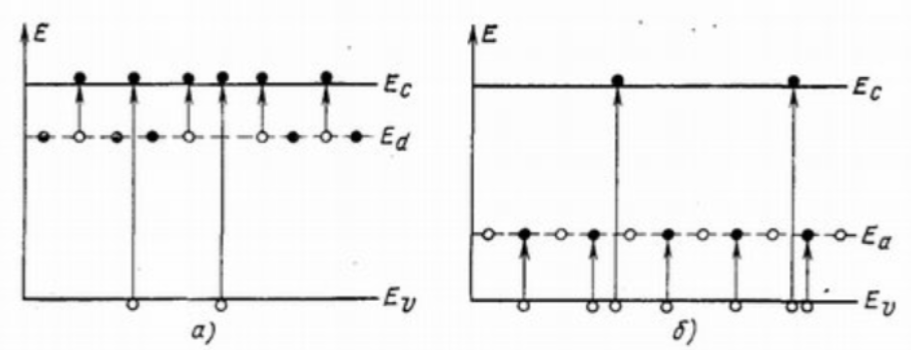
\includegraphics[width=0.7\linewidth]{Theor_pic_2.png}
    \caption{Энергетическая диаграмма донорного (а) и акцепторного (б) по-
лупроводников.}
    \label{fig:theor_pic_1}
\end{figure}

\subsection*{Теория электропроводности полупроводников}

Суммарная собственная проводимость полупроводников может быть
выражена через концентрации и подвижность электронов и дырок:

\begin{equation}
    \sigma = e(n \mu_n + p \mu_p)
\end{equation}

Проводимость примесных полупроводников, естественно тоже зависит от произведения подвижности ностилей на их концентрацию. Концентрация в данной случае складывается из концентрации собственных носителей и концентрации примесных носителей, однако при обычных температурах, в силу очень малой величины энергии донорных и акцепторных уровней, все определяется примесной проводимостью и лишь в области высоких температур, когда истощаются примесные уровни, в игру вступает собственная проводимость.

\subsection*{Уровень Ферми}
Уровень Ферми в полупроводниках не имеет такого простого физического смысла как в металлах (изменение энергии основного состояния системы при внесении в нее одной частицы), т.к он начинает зависеть от температуры => не является характеристикой вещества. Математически можно получить, что в чистых полупроводниках уровень Ферми будет находиться посередине запрещенной зоны и может смещаться при появлении примесных уровней.

\subsection*{p-n переход}

Для создания контакта электронного и дырочного полупроводников в образец вводятся донорная и акцепторная примеси соответственно. При этом концентрации доноров и акцепторов меняются так, что в одной части образец содержит доноры и обладает электронной проводимостью, а в другой части содержит акцепторы и обладачет дырочной проводимостью => в некоторой области кристалла происходит смена электропроводности с электронной на дырочную. \textit{Такой переход между материалами с электропроводностью n- и p- типа носит название p-n перехода}.

Приконтактный слой полупроводника с пониженной удельной проводимостью (обогащенный неосновными носителями заряда) называют \textit{запорным}.

\subsection*{Выпрямление тока в p-n переходе.}

Рассмотрим p-n переход, к которому приложена разность потенциалов U такая, что p-область заряжается положительно (прямое смещение). Сопротивление слоя объемного заряда перехода высокое, поэтому падение напряжения будет в основном в этой области. Поэтому при прямом смещении высота потенциального барьера понижается на eU по сравнению с равновесным состоянием, соответственно изменится и толщина запорного слоя. Понижение потенциального барьера приведет к увеличению потока основных носителей заряда. В результате этого во внешней цепи будет протекать ”прямой” ток.

В n-области появившиеся избыточные носители заряда – дырки $\Delta$p создадут вблизи контакта объемный положительный заряд. Однако через очень короткое время этот заряд будет скомпенсирован объемным зарядом основных носителей заряда – электронов, которые под действием электрического поля, созданного избыточными дырками, будут подтянуты в количестве $\Delta$n из n-области (а туда из внешней цепи).

Таким образом, во всех частях электронного полупроводника будет соблюдаться электронейтральность, но в приконтактной области к p-n переходу концентрация электронов и дырок будет повышена на $\Delta$n = $\Delta$p по сравнению с равновесным состоянием. Такое введение в полупроводник носителей заряда с помощью p − n перехода при подаче на него прямого смещения в область, где эти ноисители заряда являются неосновными, называют \textit{инжекцией}.

Аналогичные явления происходят и в p-области: сюда из n-области инжектируются электроны. Концентрация избыточных дырок и электронов в n- и p- областях:

\begin{align}
    & \Delta p = = p_n (eU \backslash kT - 1)
    & \Delta n = = n_p (eU \backslash kT - 1)
\end{align}

\textit{Т.е. с увеличением прямого смещения на p − n переходе концентрация инжектируемых неосновных носителей заряда резко возрастает, что приводит к сильному росту тока через контакт в прямом направлении}.

Если к p-n переходу приложено обратное смещение, p-область заряжена отрицательно, потенциальный барьер увеличивается на величину eU и увеличивается толщина запорного слоя объемного заряда. Меньшее количество основных носителей заряда способно преодоелеть потенциальный барьер, а значит количество неосновных носителей заряда в приконтактной области уменьшается по сравнению с равновесным состоянием. Вследствие соблюдения электронейтральности уменьшается и количество основных носителей (\textit{экстракция носителей заряда}).

\textit{Таким образом, при обратном смещении p−n перехода ток основных носителей заряда будет меньше, чем при равновесном состоянии, а ток неосновных носителей практически не изменится. Суммарный ток будет направлен от n-области к p-области и с увеличением обратного напряжения вначале будет незначительно расти, а затем стремиться к некоторой величине, называемой током насыщения}.



\subsection*{Пробой}

Существует три вида пробоя:
\begin{itemize}
    \item туннельный пробой (эффект Зенера);
    \item лавинный пробой;
    \item тепловой пробой.
\end{itemize}

Туннельный пробой имеет место, когда напряженность электрического поля принимает такие значения, что может происходить туннельный переход из валентной зоны полупроводника с электропроводностью одного типа в зону полупроводника с электропроводностью другого типа. Можно наблюдать при напряжениях ниже 6 В. 

Лавинный пробой происходит из-за образования носителей заряда ввиду ударной ионизации атомов полупроводника. Если напряженность электрического поля достаточно велика, то электроны начинают иметь энергию, достаточную для того, чтобы выбивать другие электроны из атомов кристаллической решетки. Из-за этого процесса происходит быстрое нарастание обратного тока.

Тепловой пробой обусловен нагревом перехода. За счет тепловой энергии происходит генерация пар электрон – дырка. Благодаря этому происходит увеличение обратного тока и дальнейшее увеличение температуры, из-за чего изменяется структура кристалла и он выводится из строя.

\subsection*{Типы диодов и их применение}

Основные типы полупроводниковых диодов:

\begin{itemize}
    \item Полупроводниковый;
    \item Туннельный;
    \item Шоттки;
\end{itemize}

Полупроводниковый диод основан на p-n переходе и использует его нелинейную ВАХ при подаче разности потенциалов на электроды. Массово используется для всевозможных задач. (рис. \ref{fig:theor_diods})

Туннельный диод развивает идею предыдущего (тот же p-n) переход, однако оба полупроводника сильно легированы, в результате чего смещение их зон настолько сильное, что может наблюдаться отрицательное дифференциальное сопротивление. Применяется в усилителях, генераторах и т.п (рис. \ref{fig:theor_diod_0}) 

Диод Шоттки основан на контакте металл-полупроводник: в качестве барьера Шоттки используется переход металл-полупроводник, в отличие от обычных диодов, где используется p-n-переход. Переход металл-полупроводник обладает рядом особенных свойств (отличных от свойств полупроводникового p-n-перехода). К ним относятся: пониженное падение напряжения при прямом включении, высокий ток утечки, очень маленький заряд обратного восстановления. Последнее объясняется тем, что по сравнению с обычным p-n-переходом у таких диодов отсутствует диффузия, связанная с инжекцией неосновных носителей, то есть они работают только на основных носителях. Применяется везде где требуется минимальное падение напряжения - в блоках питания, стабилизаторах напряжения. (рис. \ref{fig:theor_diods})

\begin{figure}[H]
    \centering
    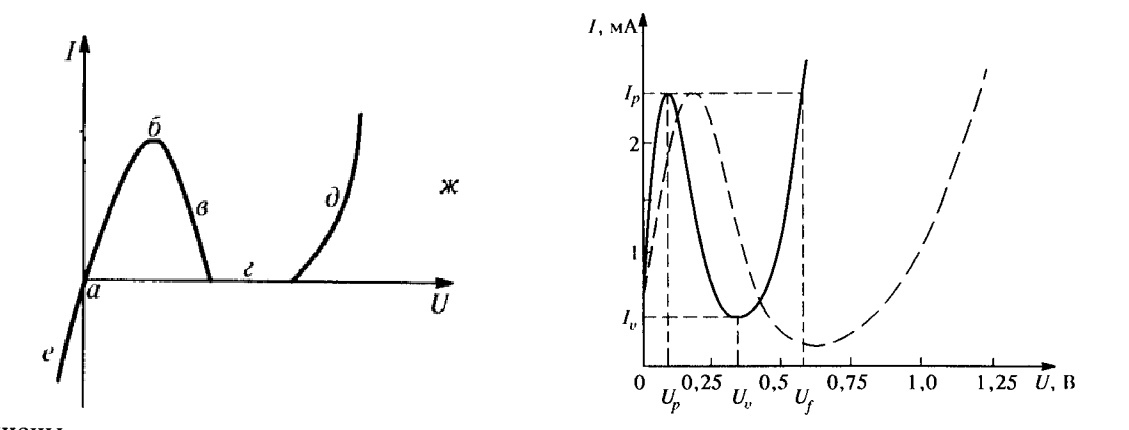
\includegraphics[width=0.7\linewidth]{Theor_diod_1.png}
    \caption{Теоретическая и практическая ВАХ для туннельного диода.}
    \label{fig:theor_diod_0}
\end{figure}

\begin{figure}[H]
    \centering
    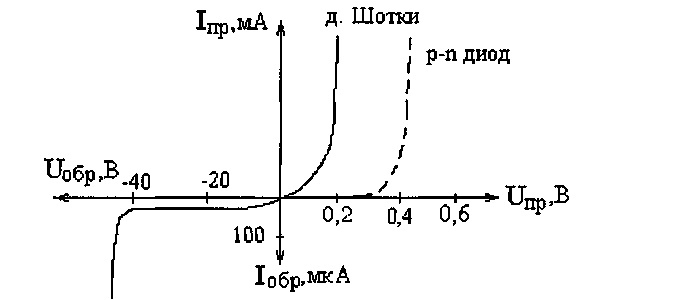
\includegraphics[width=0.7\linewidth]{Shottki_theor.jpg}
    \caption{Теоретические ВАХ для обычного полупроводникового диода и диода Шоттки.}
    \label{fig:theor_diods}
\end{figure}


\subsection*{Экспериментальная установка}

\begin{minipage}[H]{.5\linewidth}
    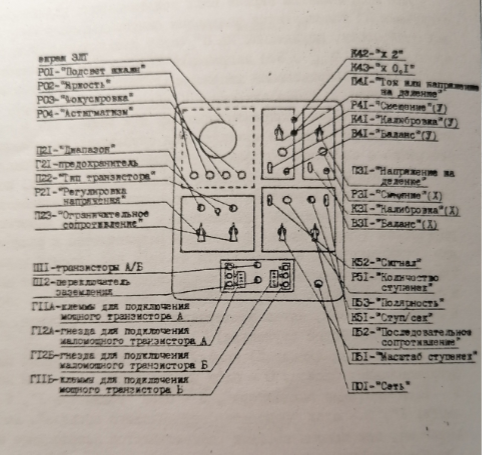
\includegraphics[width = 1\linewidth]{PNCHT_theor.png}
    \captionof{figure}{Схема характериографа}
\end{minipage}
\begin{minipage}[H]{.5\linewidth}
    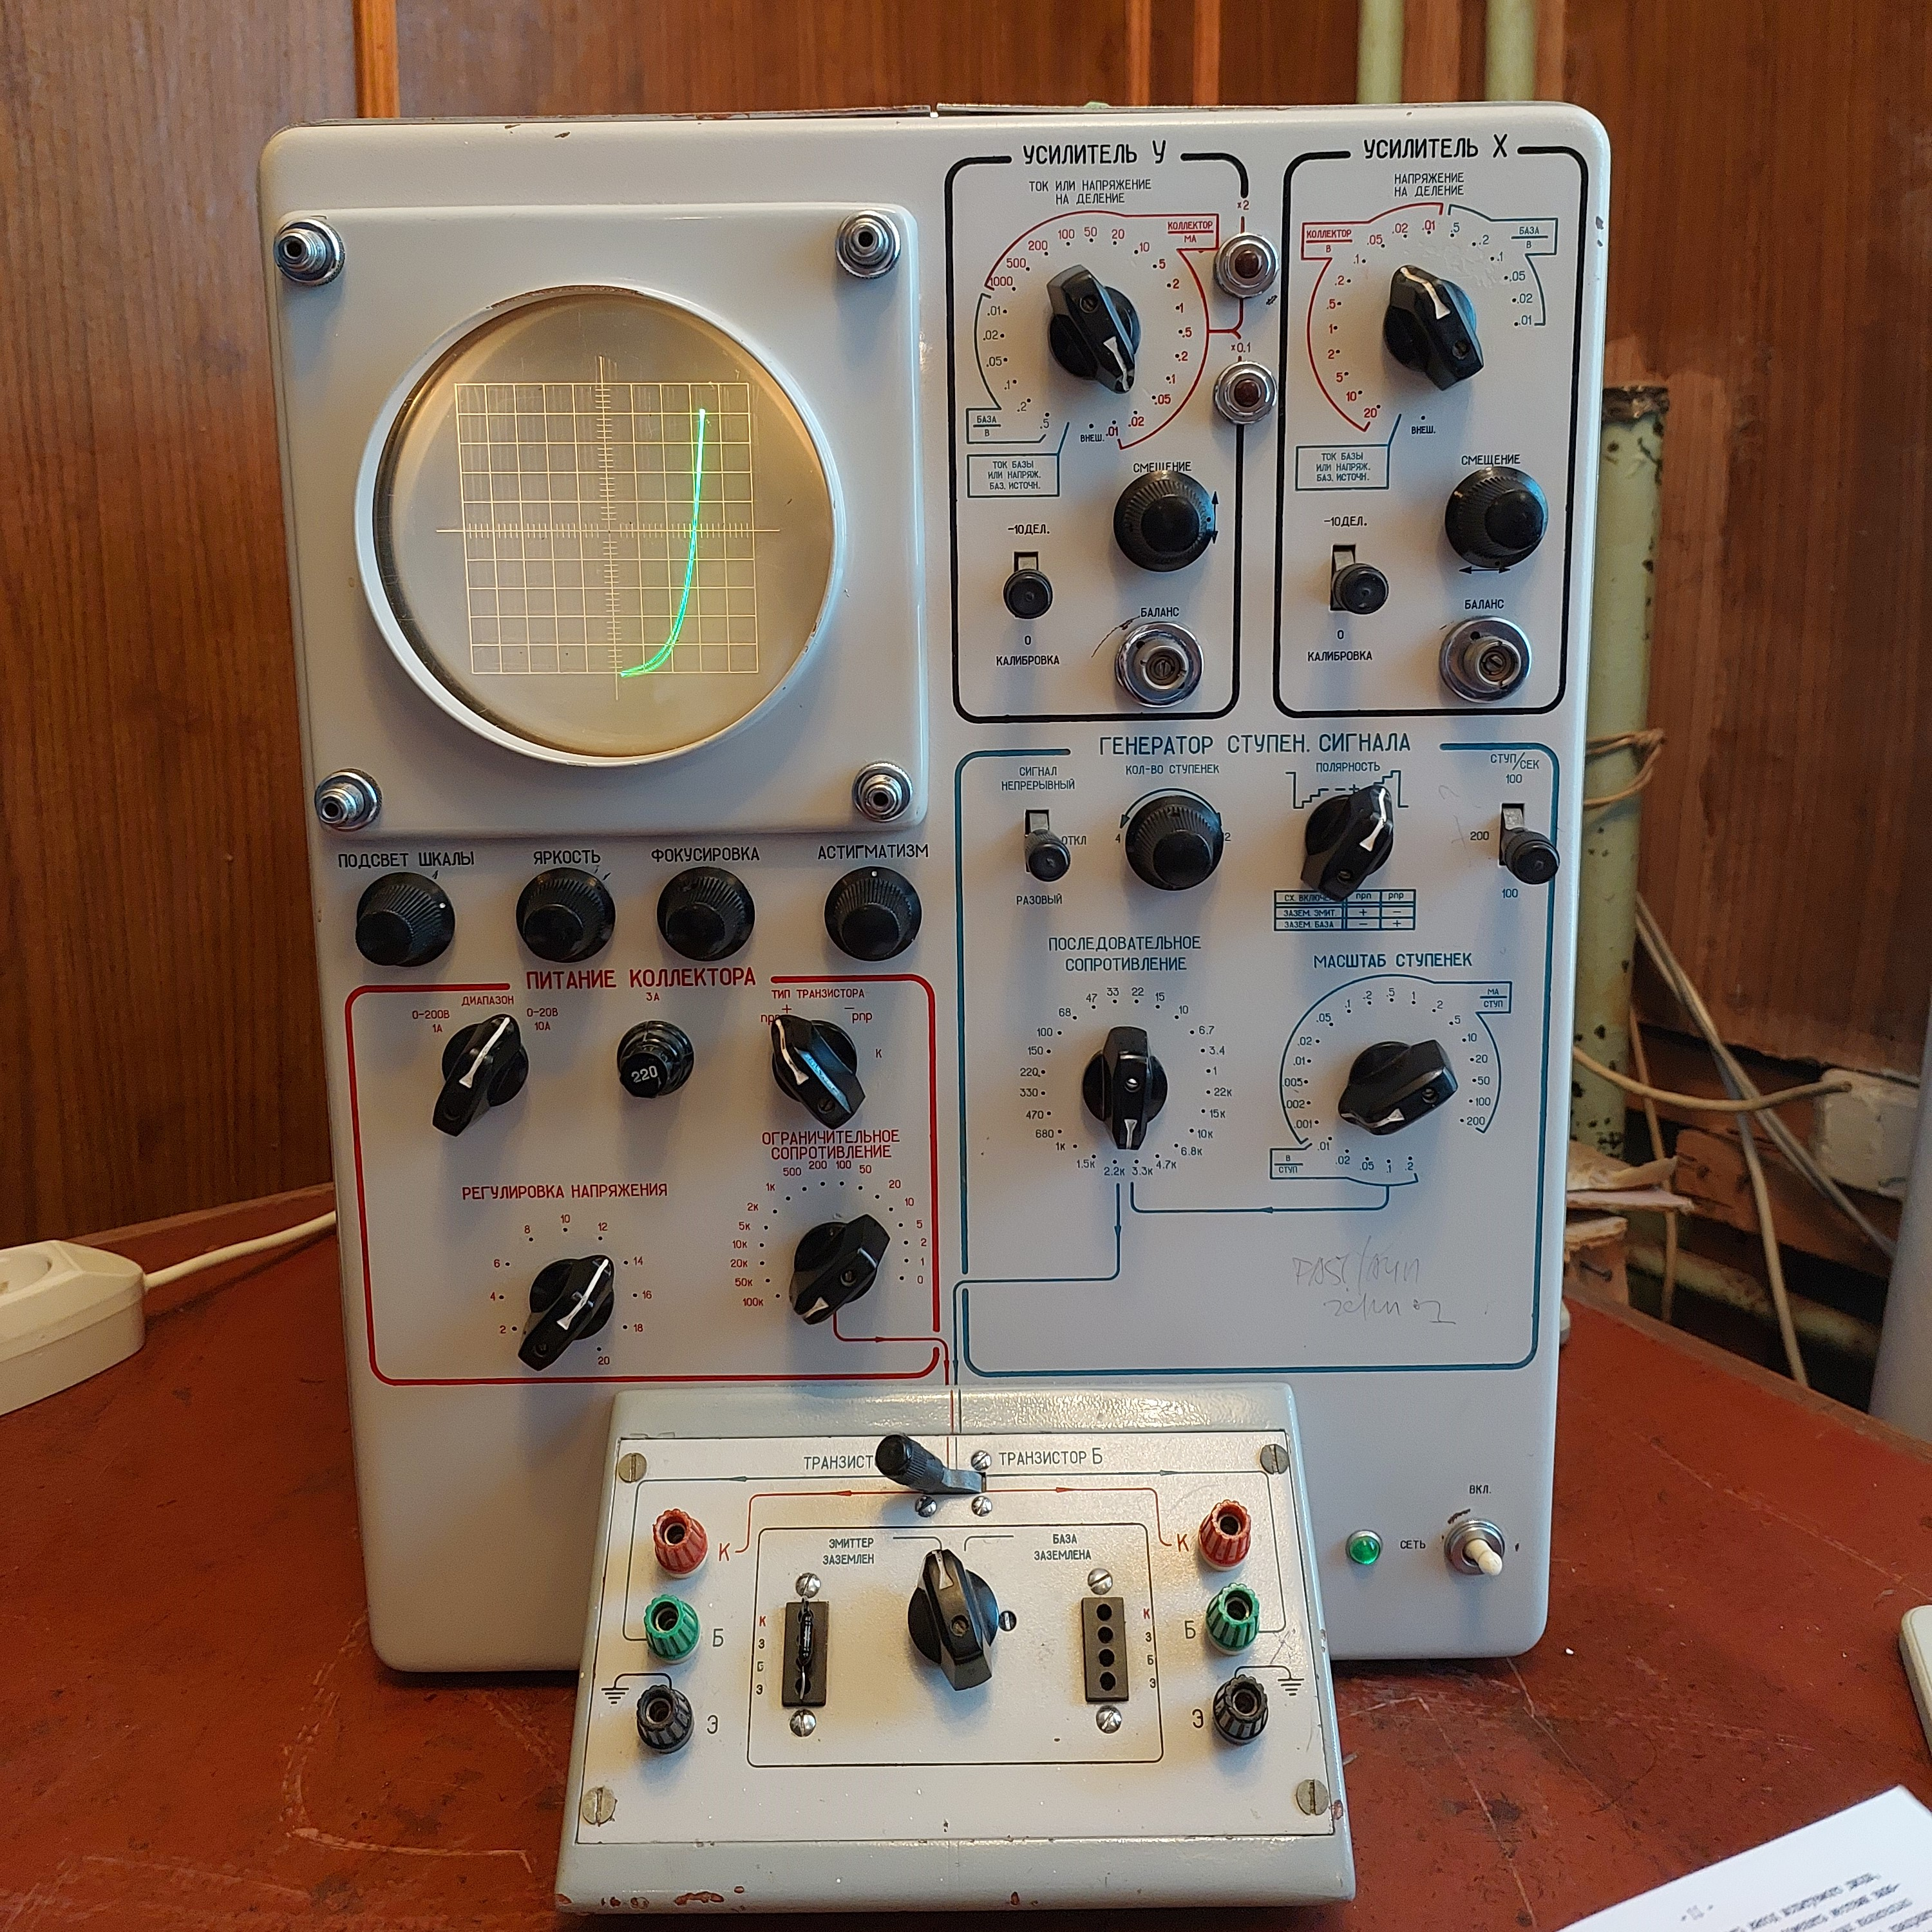
\includegraphics[width = 1\linewidth]{PNCHT_real.jpg}
    \captionof{figure}{Вид установки}
\end{minipage}

% \begin{figure}[H]
%     \centering
%     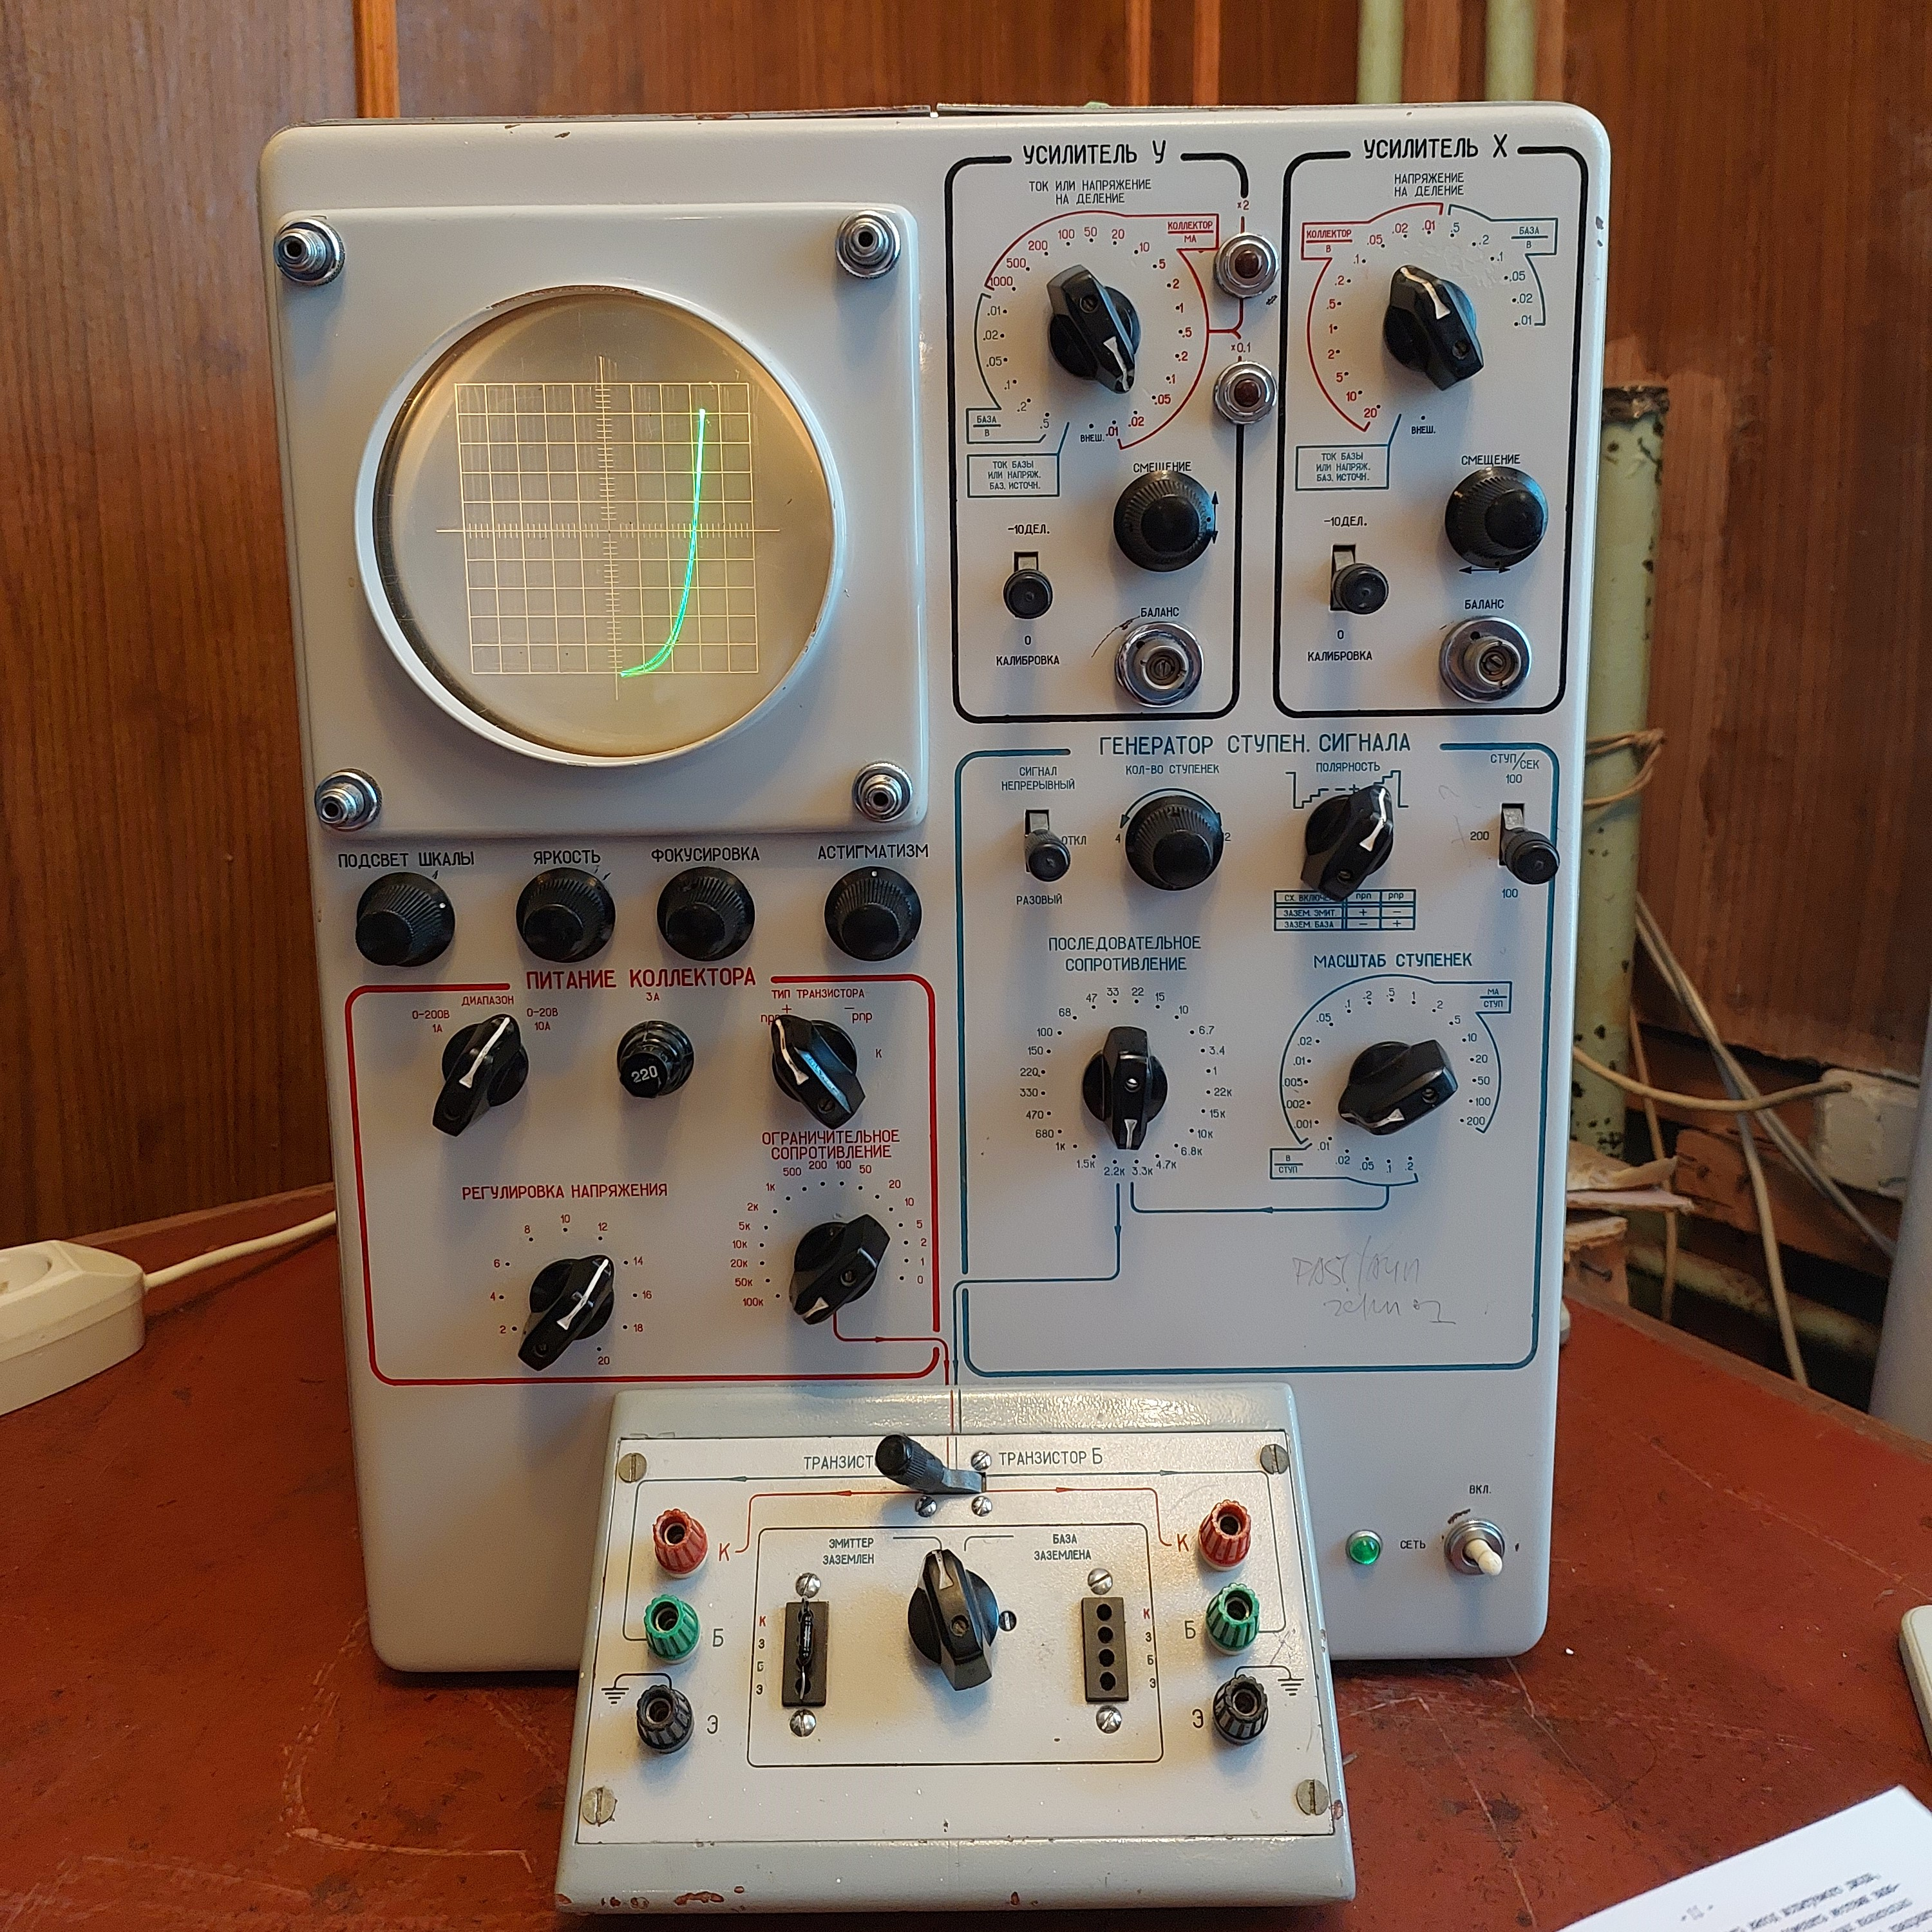
\includegraphics[width=0.7\linewidth]{PNCHT_real.jpg}
%     \caption{Характериограф}
% \end{figure}

% \begin{figure}[H]
%     \centering
%     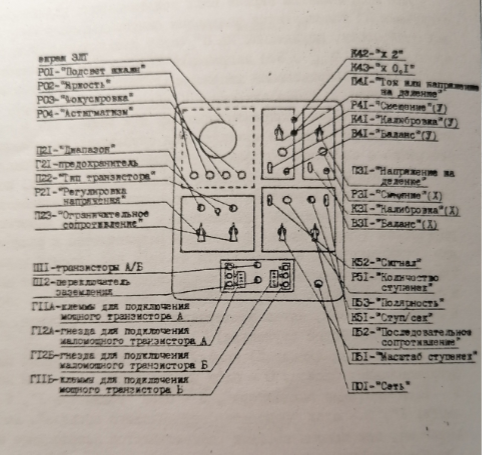
\includegraphics[width=0.7\linewidth]{PNCHT_theor.png}
%     \caption{Схема характериографа}
% \end{figure}

ПНХТ (прибор для наблюдения характеристик транзисторов) предназначен для визуального наблюдения и измерения статических характеристик полупроводниковых приборов. На передней панели ПНХТ можно выделить 6 функциональных блоков: 0 – блок визуализации, 1 – блок коммутации, 2 – блок ”питание коллектора”, 3 – блок ”усилитель X”, 4 – блок ”усилитель Y”, 5 – блок ”генератор ступенчатого сигнала” (не используется в данной работе).

Для получения на экране ПНХТ вольтамперных характеристик исследуемых приборов, используются полуволны синусоидальнго напряжения требуемой полярности, подаваемые на полупроводниковый прибор через последовательный резистор с сопротивлением rпк. Это напряжение используется в качестве сигнала аргумента (развертывающее напряжение).

\section*{Результаты измерений и обработка данных}
\subsection*{Диод 1.}

Снимем ВАХ первого диода с экрана ПНХТ. Цена деления на выходе X в 0.02 мА, а на выходе Y в 0.1 В. Получим следующие графики для прямой и обратной ветвей.

\begin{figure}[H]
    \centering
    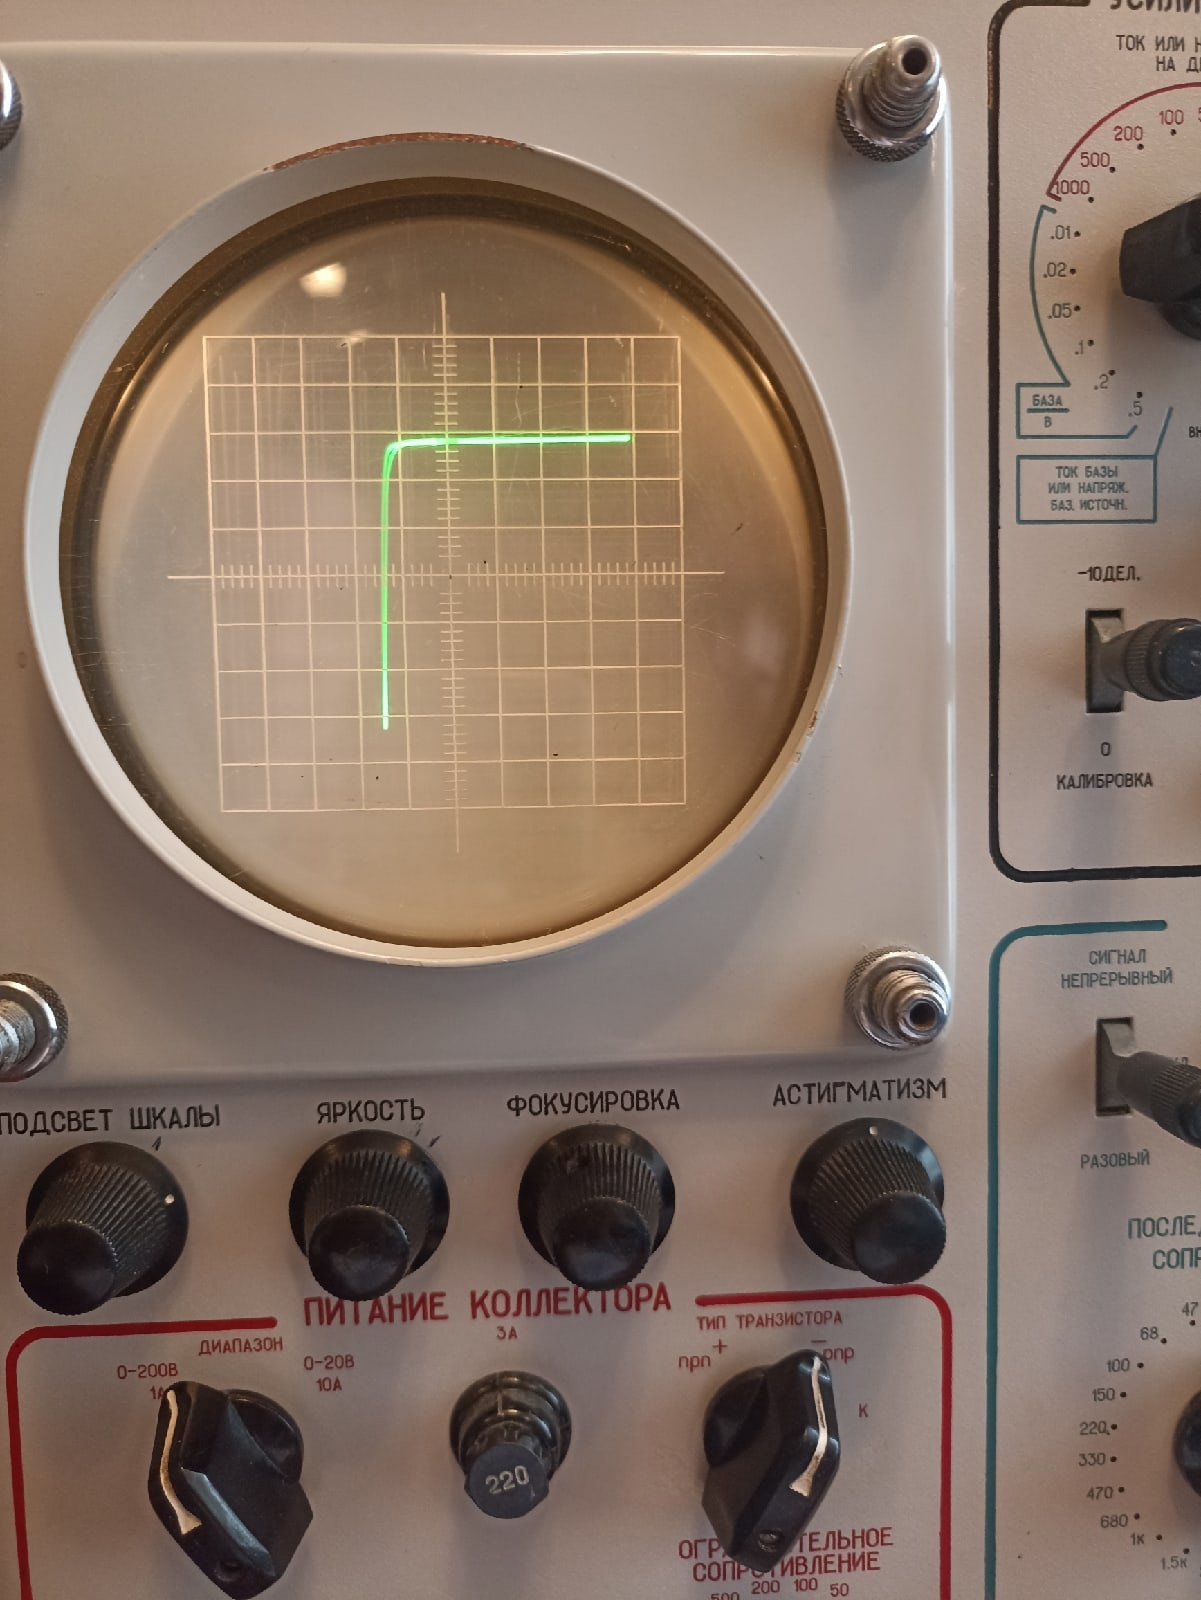
\includegraphics[width=0.4\linewidth]{diod12.jpg}
    \caption{ВАХ для обратной ветви диода 1.}
\end{figure}

\begin{figure}[H]
    \centering
    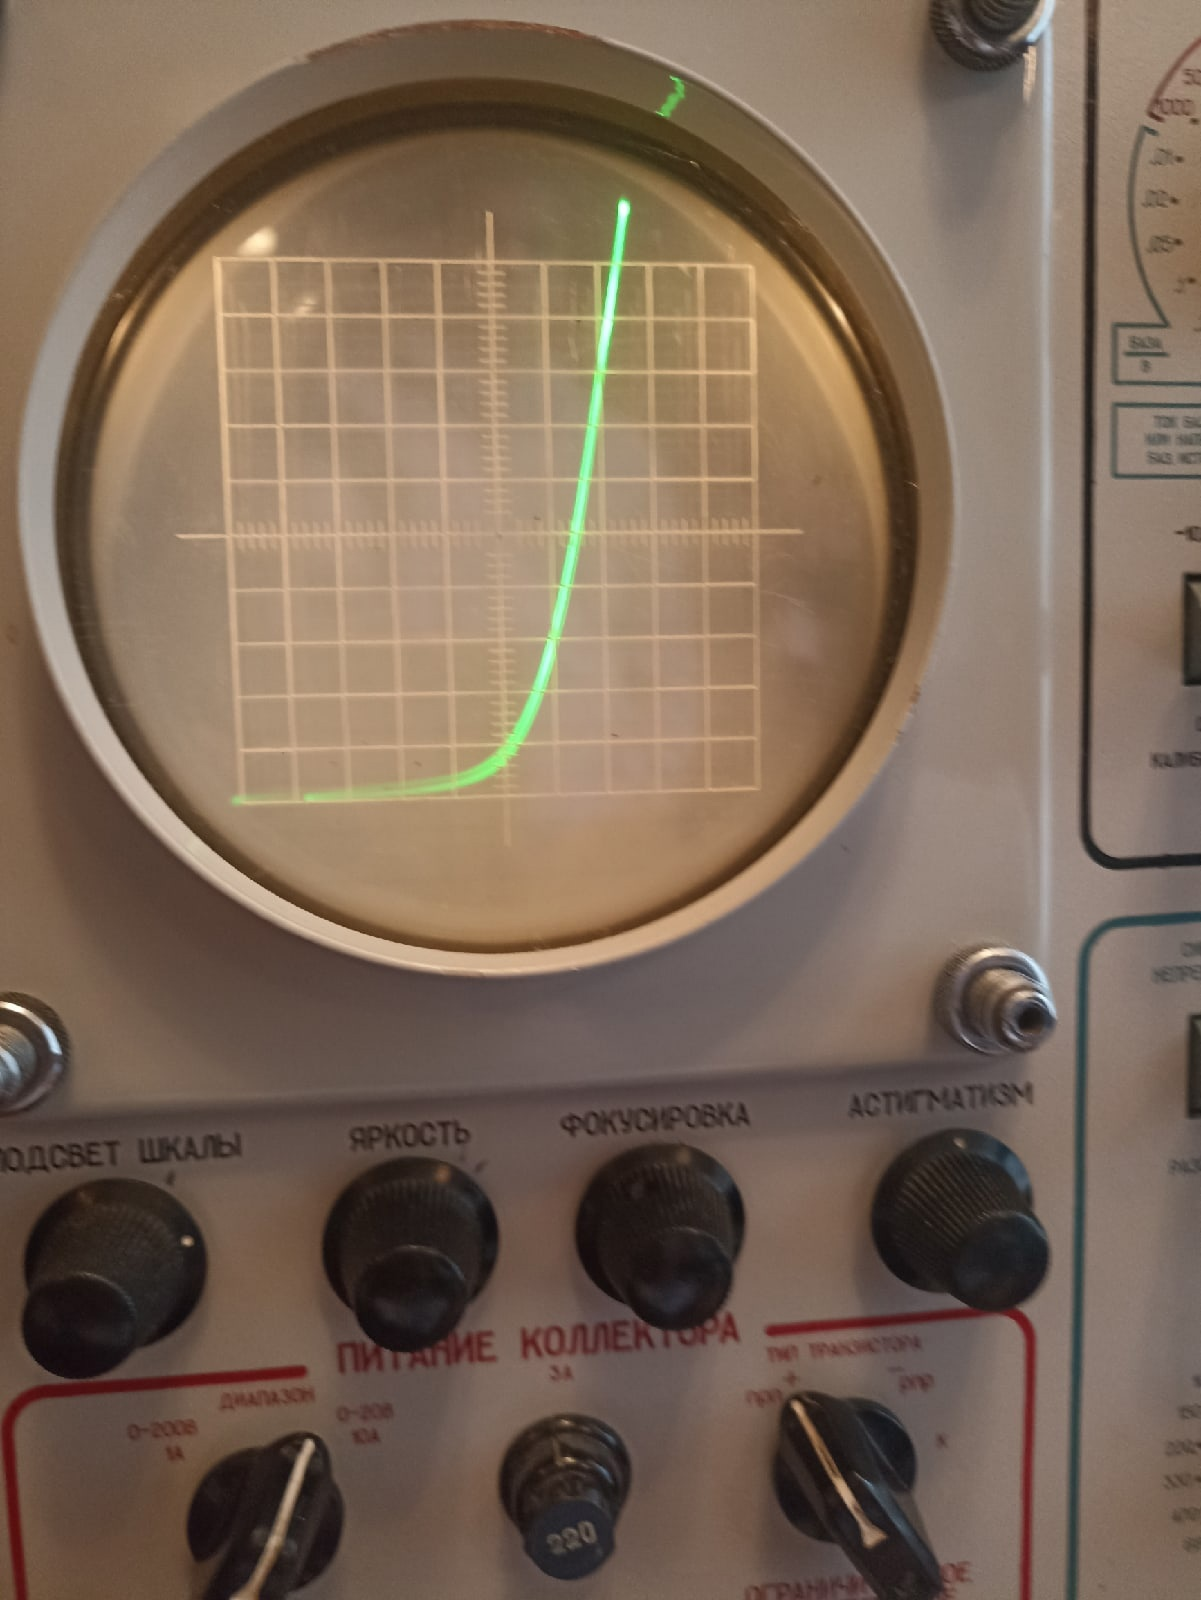
\includegraphics[width=0.4\linewidth]{diod11.jpg}
    \caption{ВАХ для прямой ветви диода 1.}
\end{figure}


Из полученной ВАХ и теоретического рисунка \ref{fig:theor_diods} определяем, что диод 1 - это диод Шоттки.


Выполним пункт 5 задания. Аппроксимируем полученные экспериментальные точки для прямой ветви экспоненциальной зависимостью (\ref{eq1}), получим следующий график зависимости.

\begin{figure}[H]
    \centering
    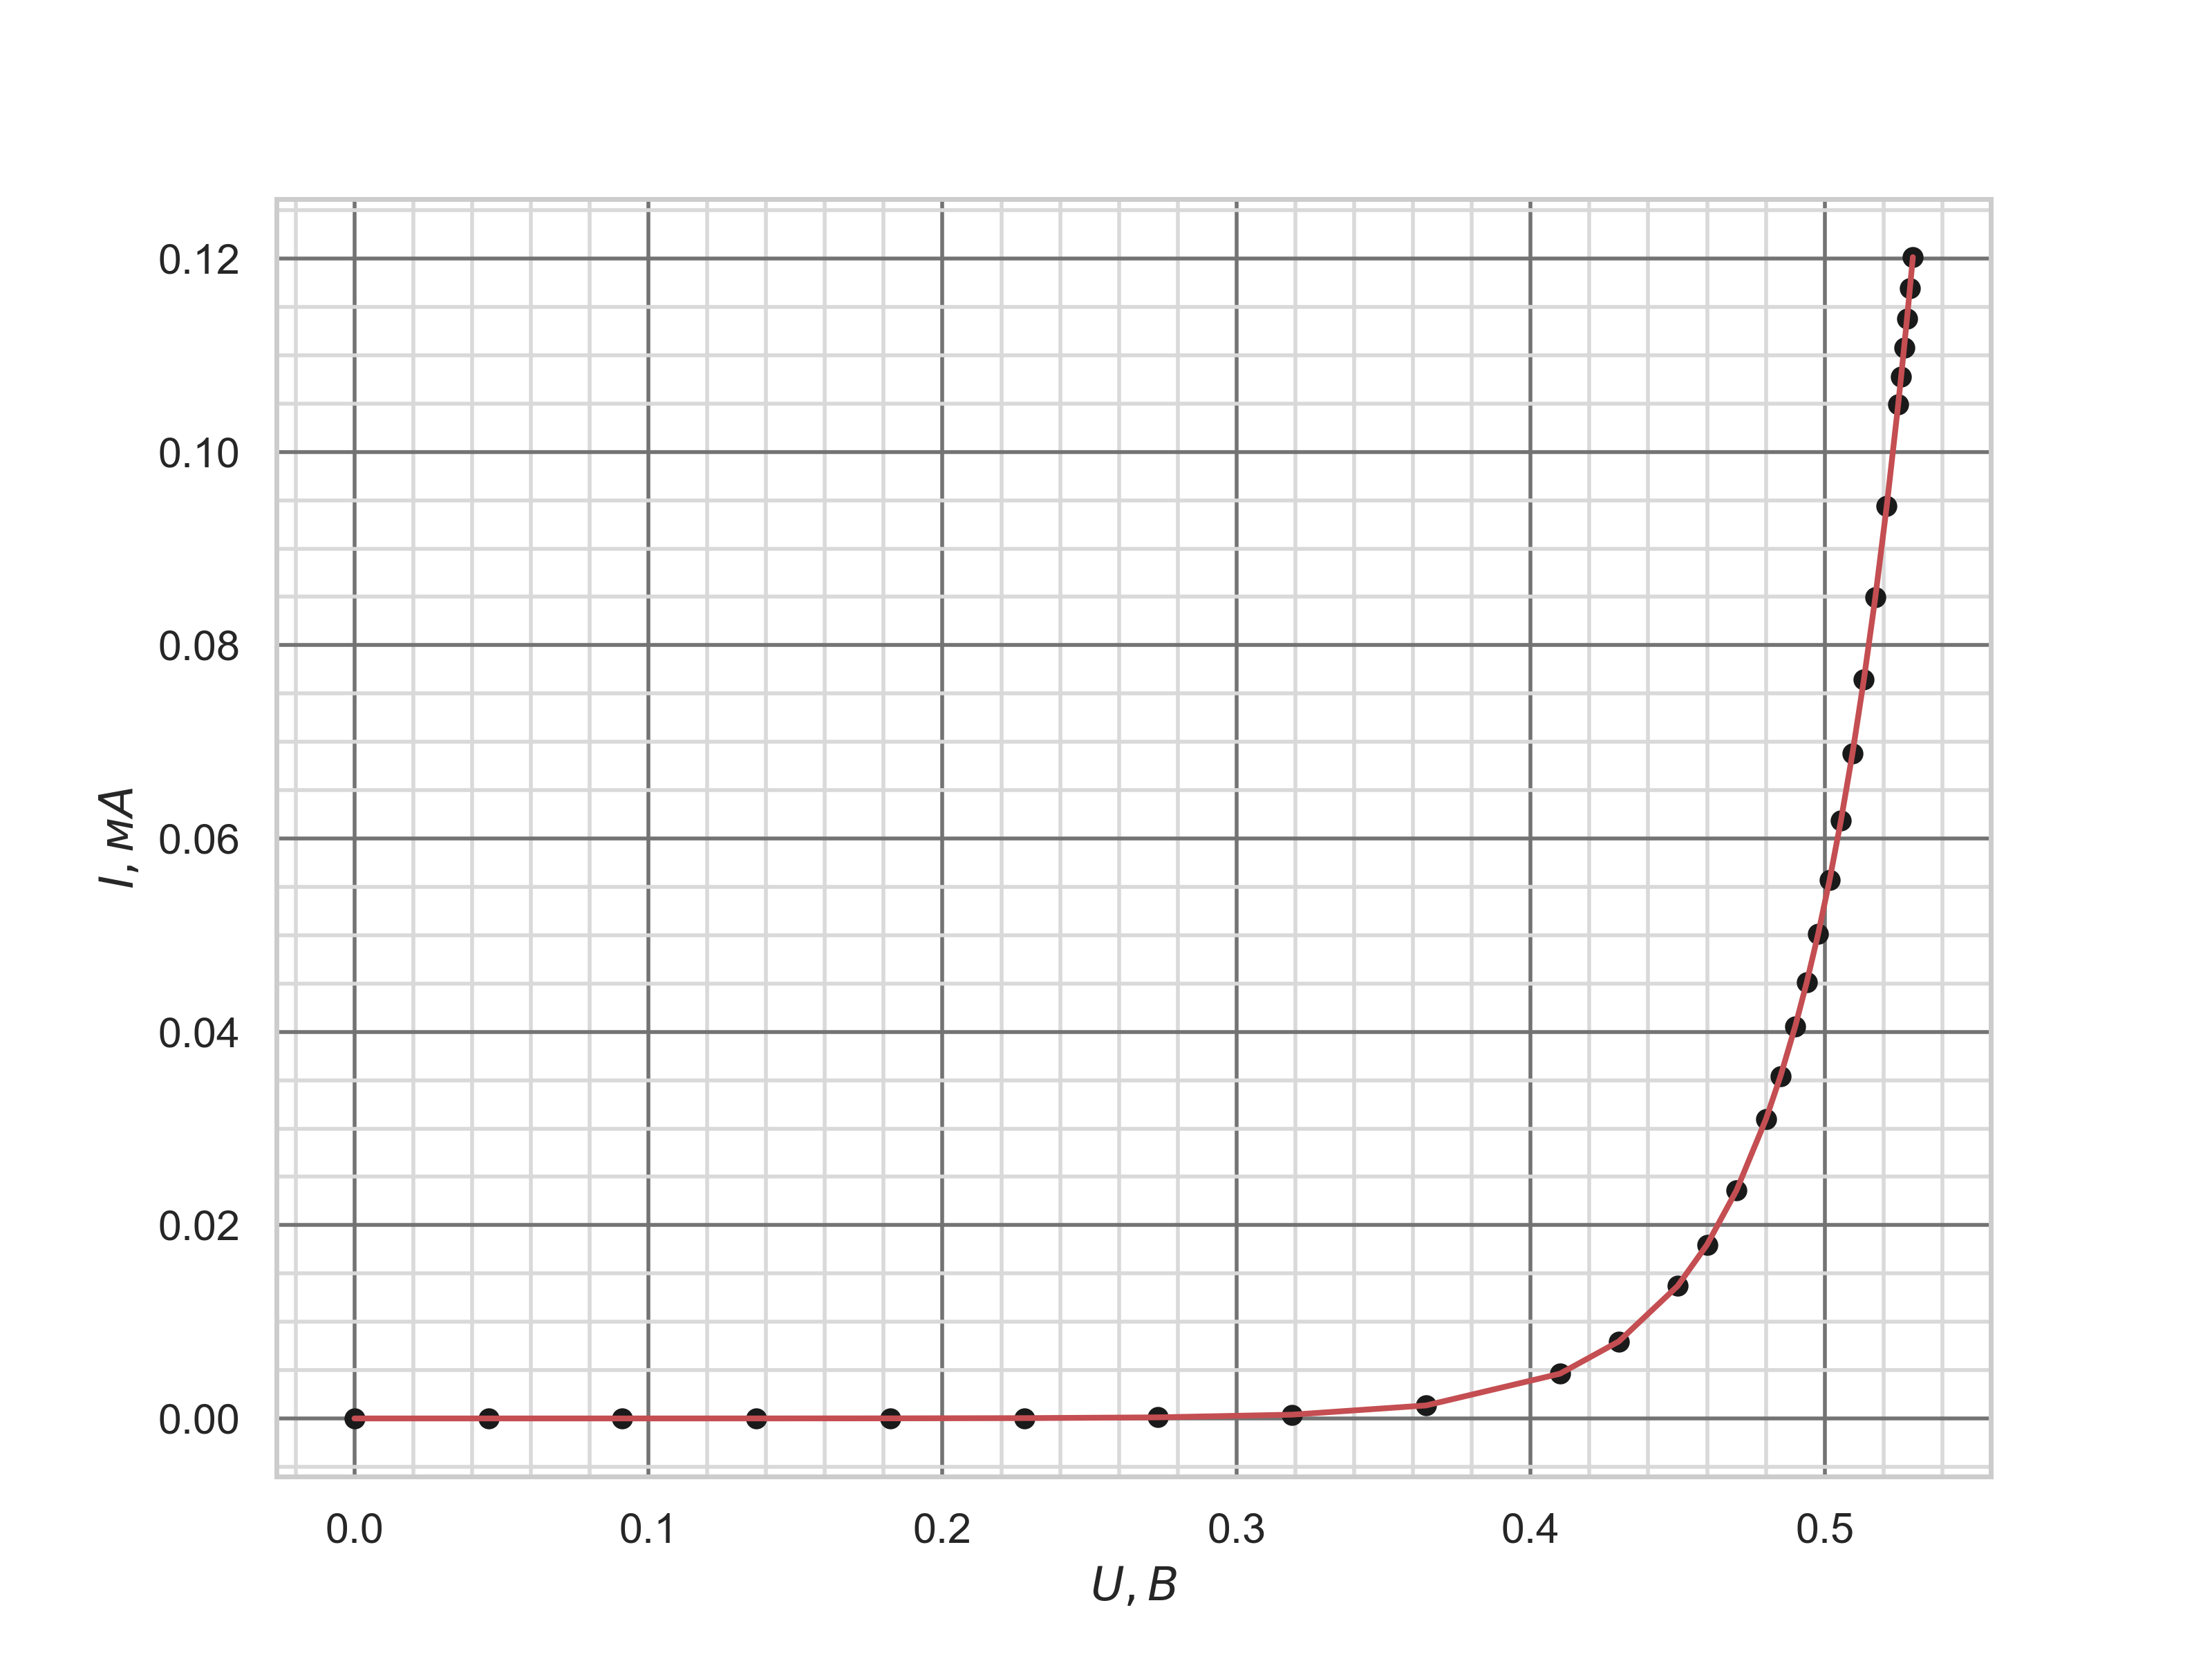
\includegraphics[width=0.7\linewidth]{Diod_1_approximation.png}
    \caption{Аппроксимация экспериментальных точек экспоненциальной зависимостью.}
\end{figure}

Получаем следующие значения для коэффициента неидеальности $\theta$ и тока насыщения $I_{d0}$:
\[
\Theta_1 = 1.4, \, I^1_{d0} = 7 \cdot 10^{-5} \text{ мкА}
\]

\newpage

\subsection*{Диод 2.}
Проделаем аналогичные выкладки для второго диода. 

Снимем ВАХ для диода 2:

\begin{figure}[H]
    \centering
    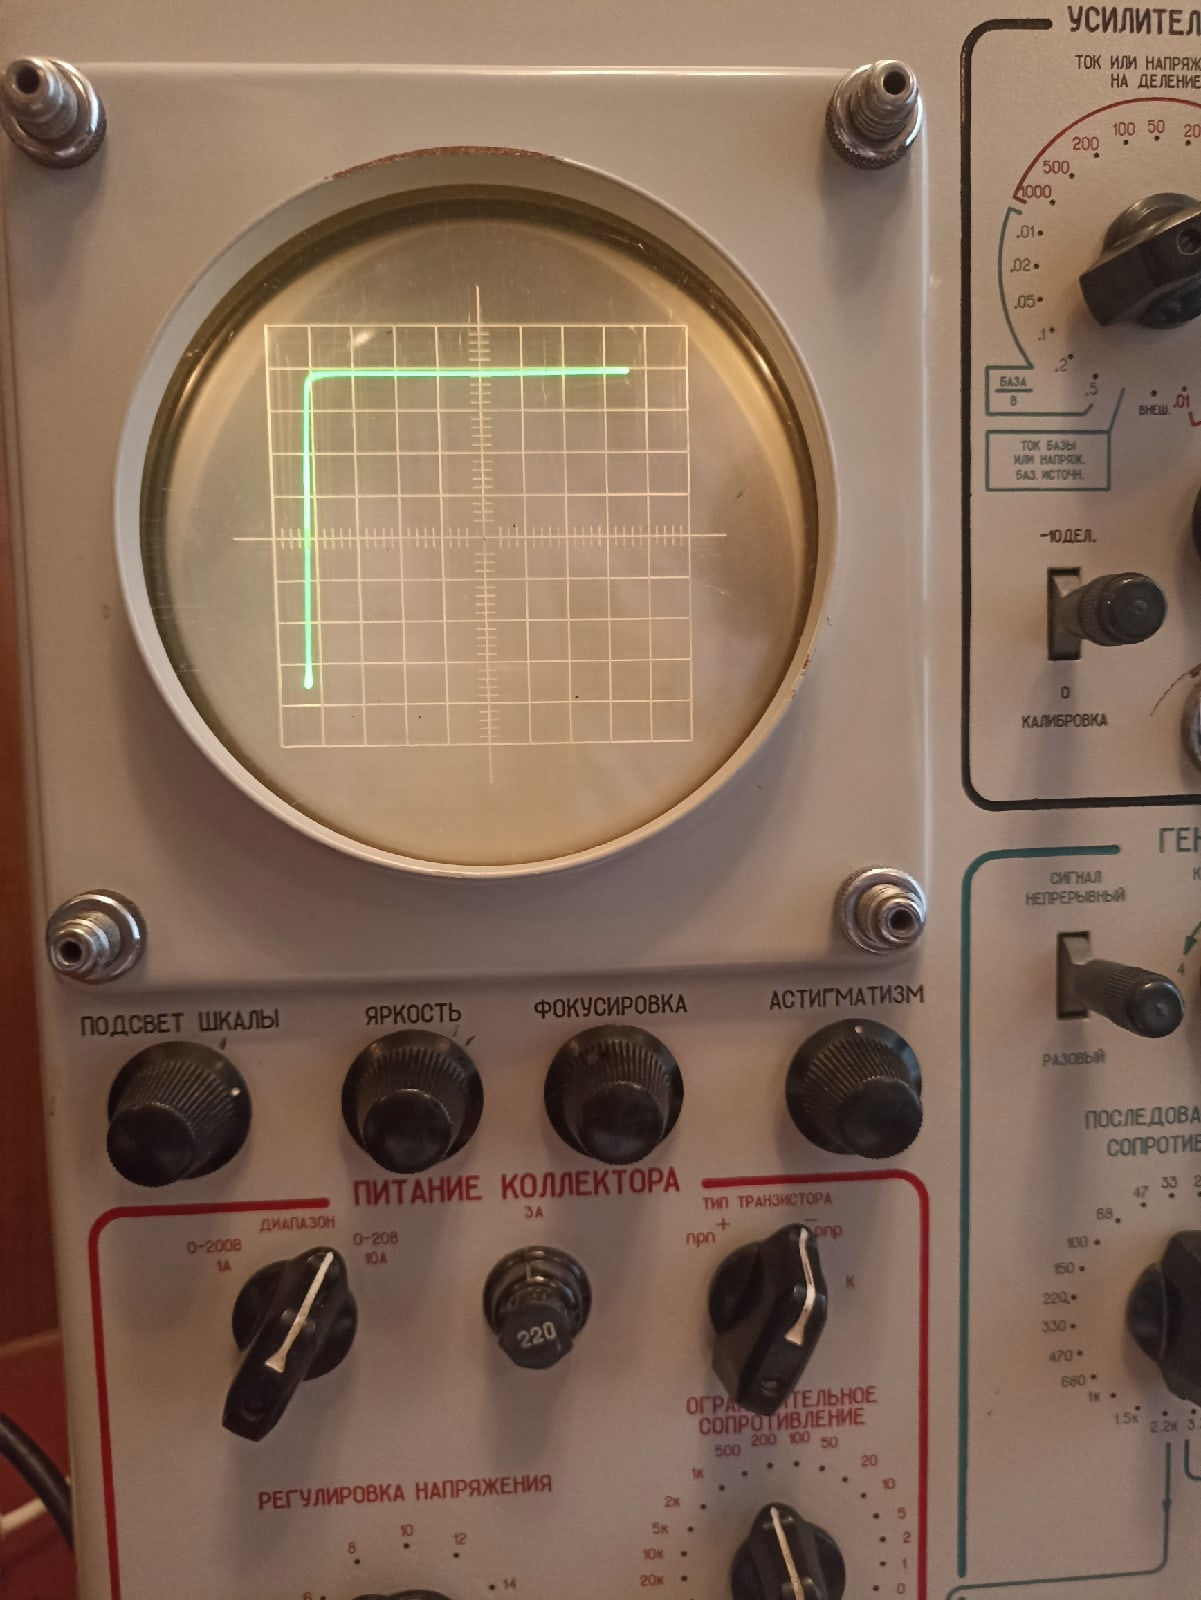
\includegraphics[width=0.4\linewidth]{diod22.jpg}
    \caption{ВАХ для обратной ветви диода 1.}
\end{figure}

\begin{figure}[H]
    \centering
    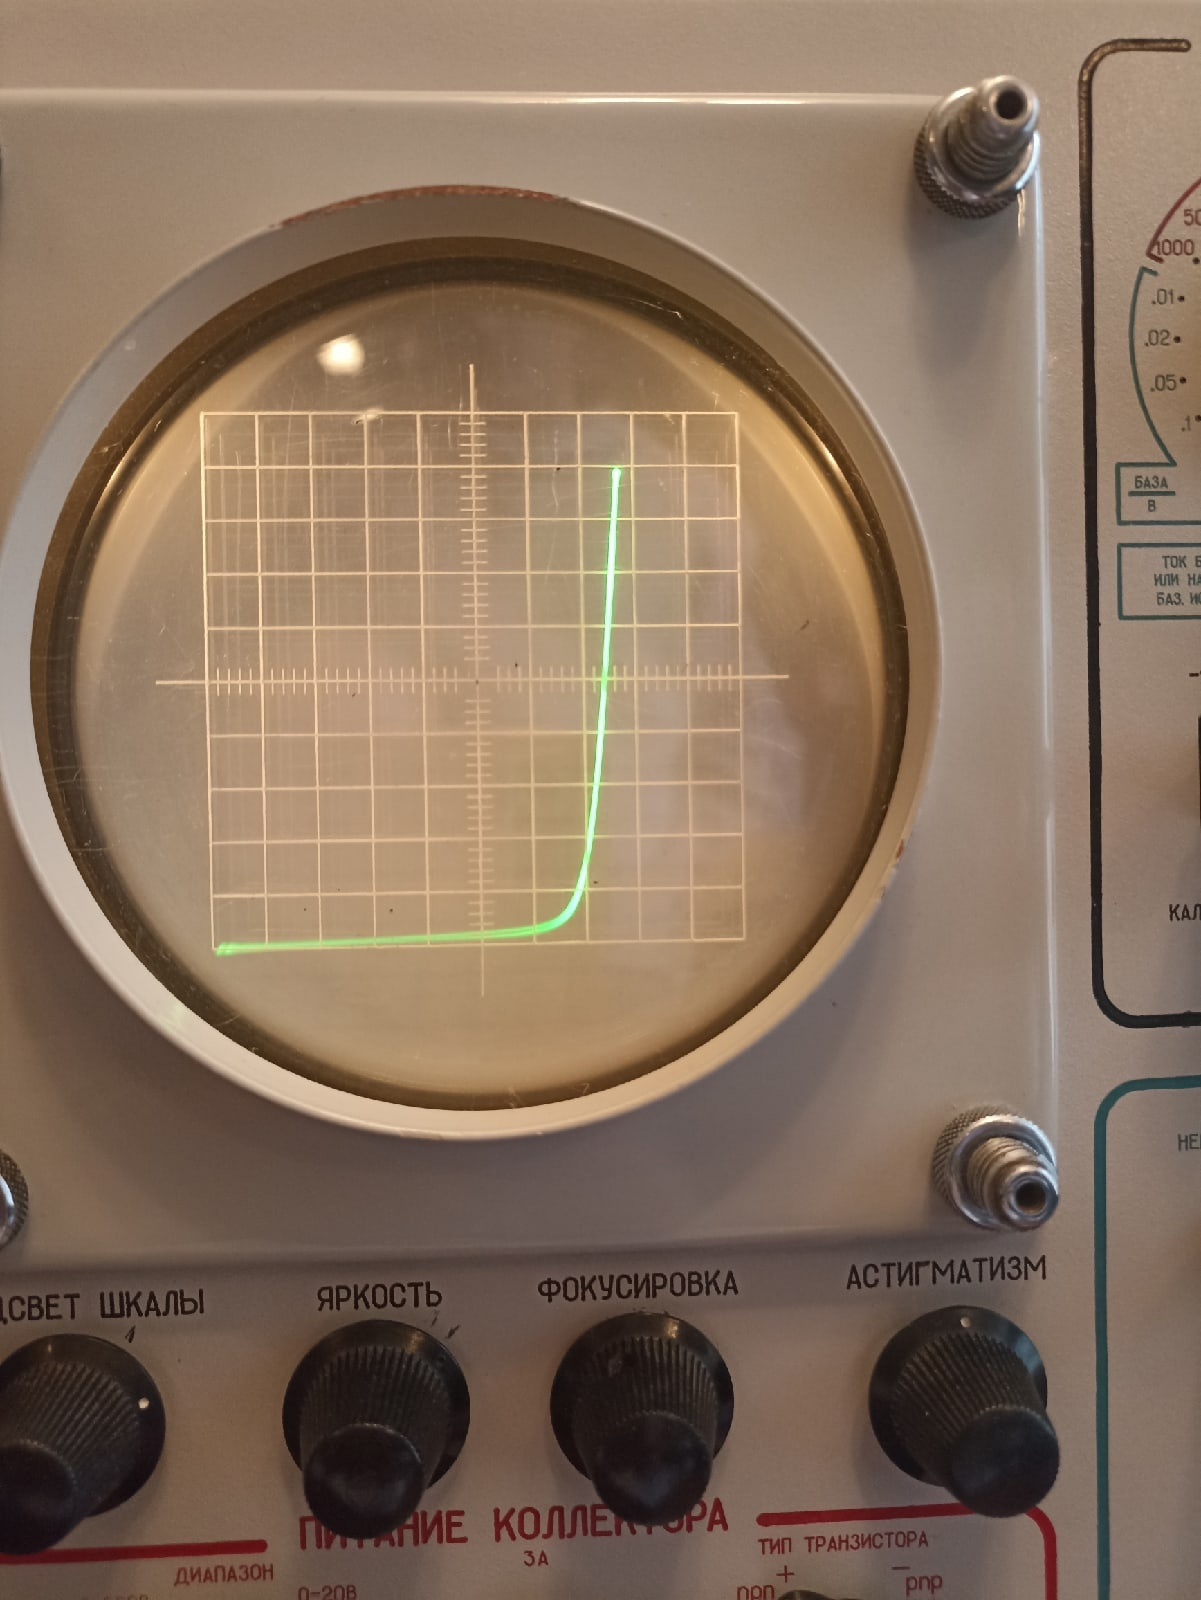
\includegraphics[width=0.4\linewidth]{diod21.jpg}
    \caption{ВАХ для прямой ветви диода 1.}
\end{figure}

Из полученной ВАХ и теоретического рисунка \ref{fig:theor_diods} устанавливаем, что диод 2 - обычный p-n диод.

Рассчитаем токи насыщения, считая диоды идеальными, по формуле:
\begin{equation}
\label{eq1}
    I = I_{d_0}[exp(\frac{U}{\varphi_T})-1]
\end{equation}

Построим зависимость $I_{d_0}(I)$:

\begin{figure}[H]
    \centering
    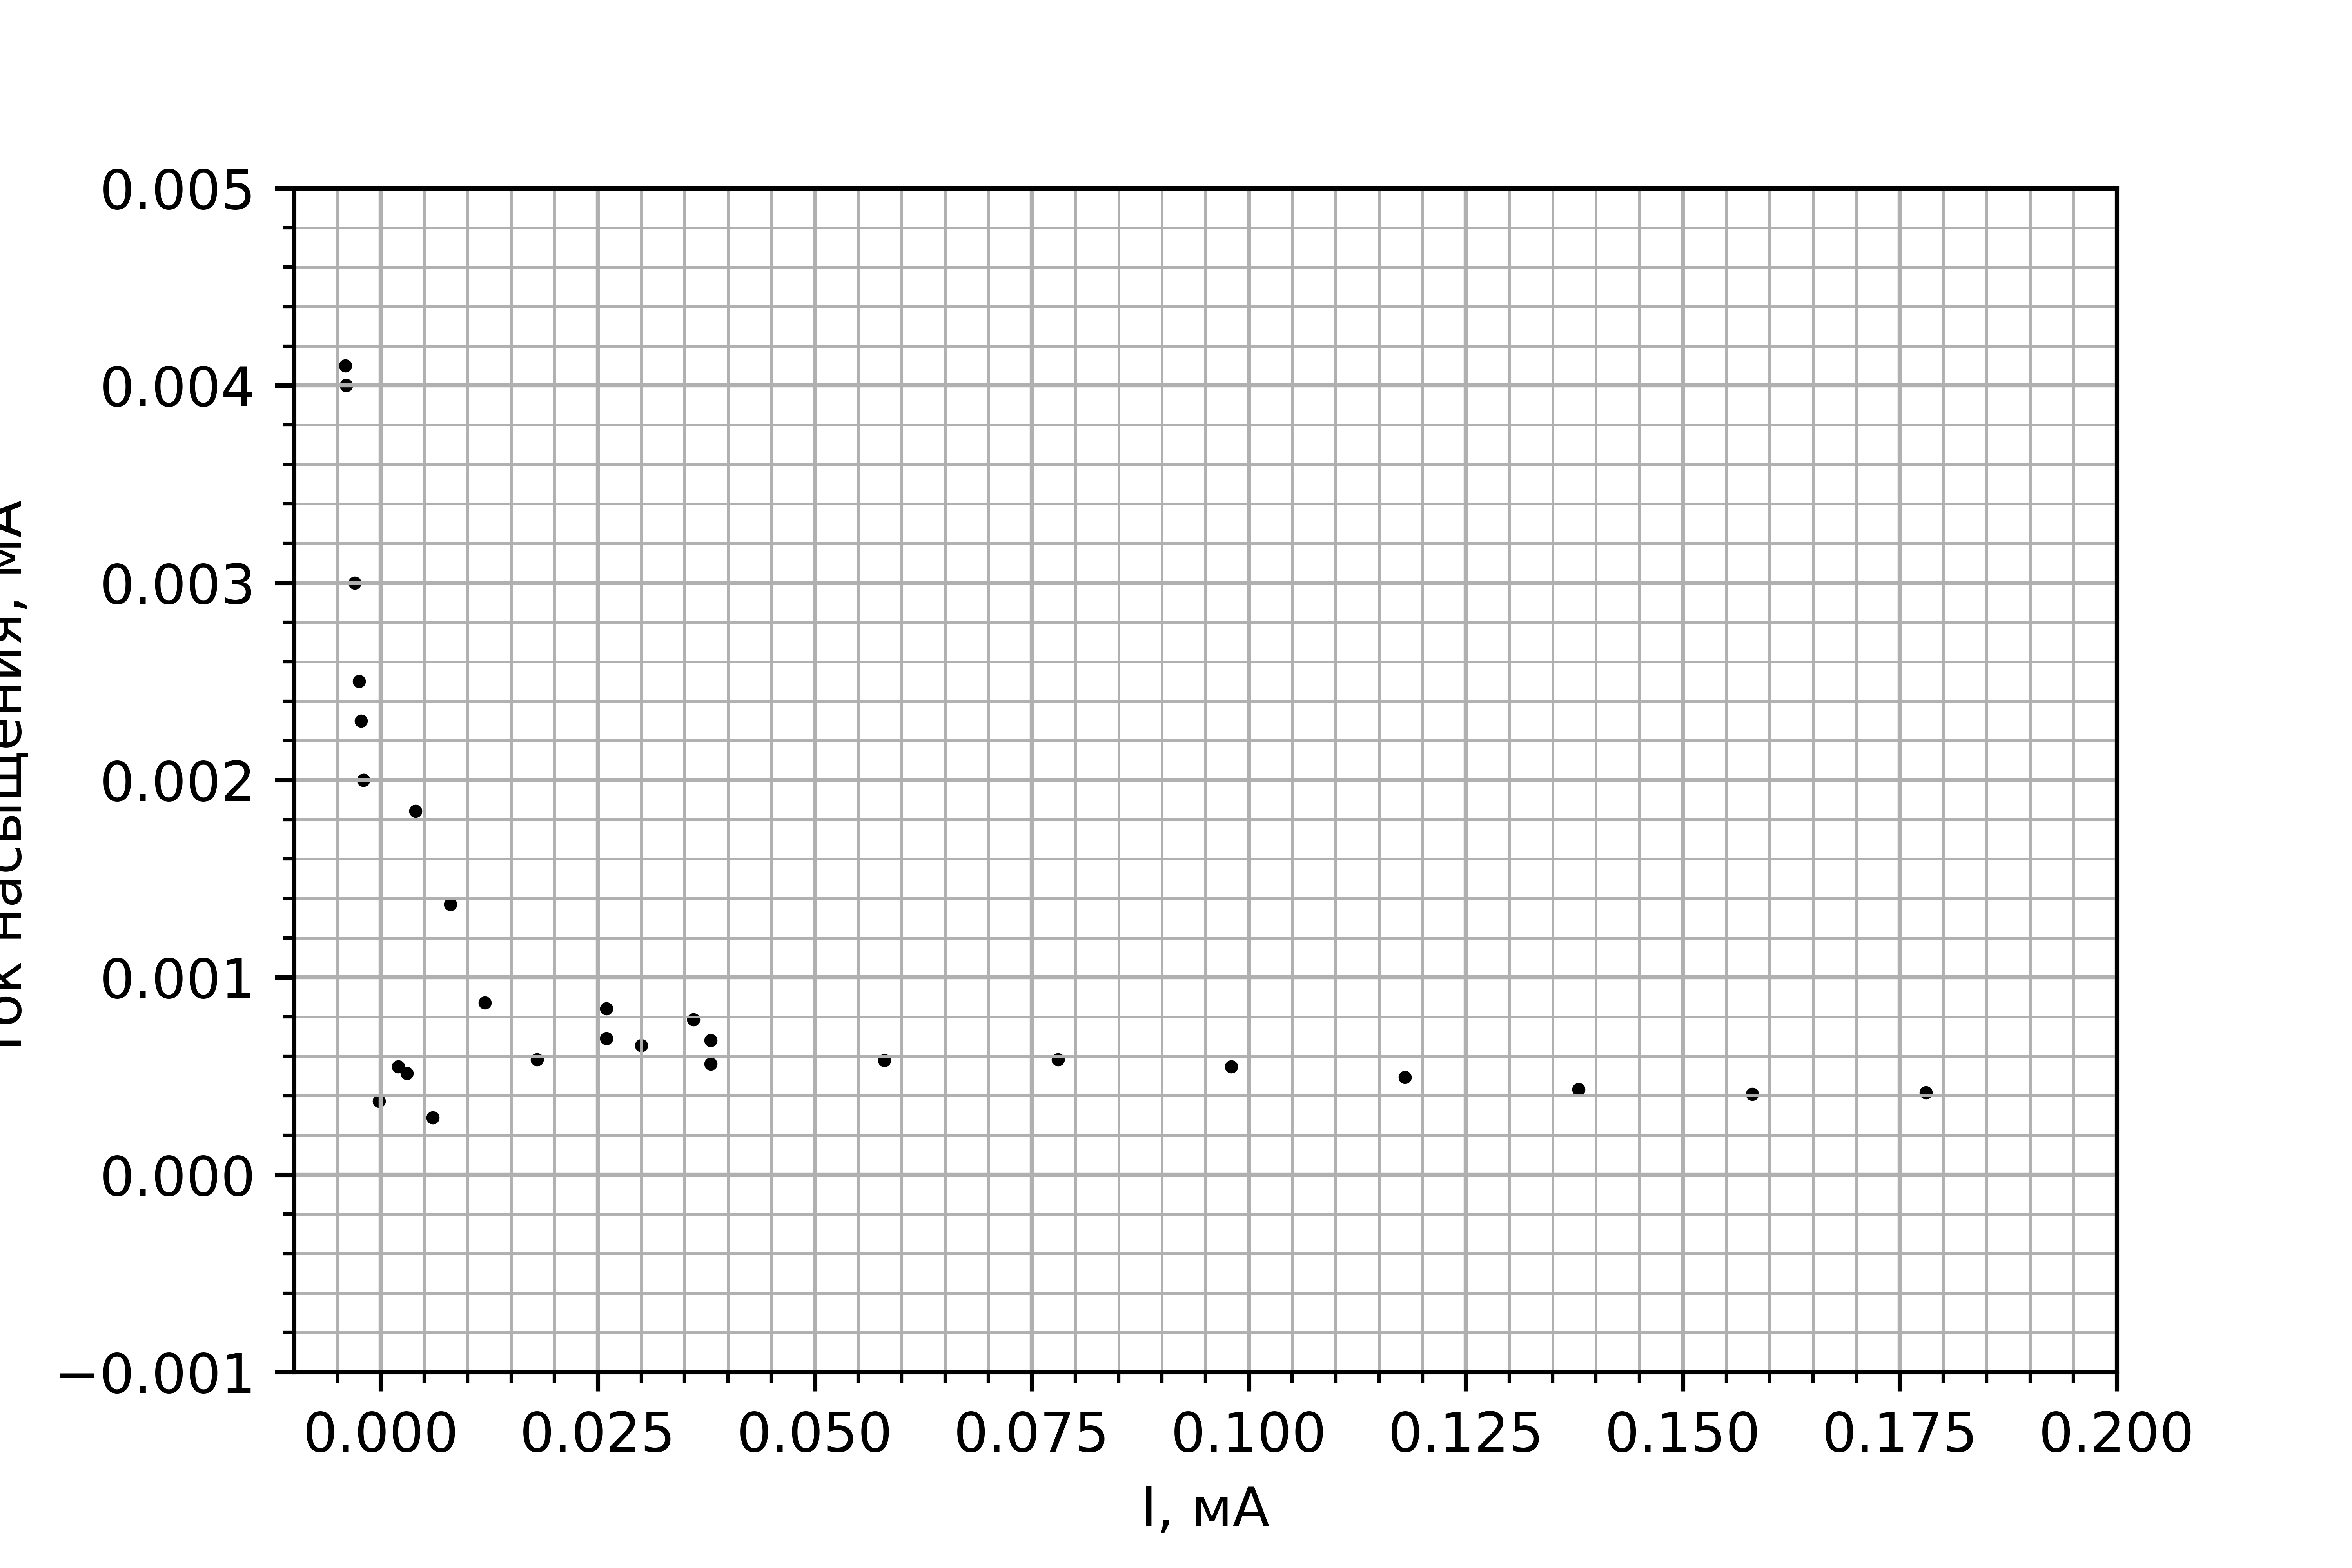
\includegraphics[width=0.7\linewidth]{Id0(I)_d2.png}
    \caption{Зависимость тока насыщения $I_{d0}$ от тока через диод $I_d$ для диода 2.}
\end{figure}

Далее учтем неидеальность диодов и аппроксимируем полученные ВАХ формулой:
\begin{equation}
\label{form: I_d0}
    I = I_{d_0}[exp(\frac{U}{\Theta\cdot\varphi_T})-1]
\end{equation}

Аппроксимация проводилась аналогичными методами, как и для диода 1.

Таким образом получены характерные параметры:
\begin{center}
    $I^2_{d_0}$ = 4,4 мкА , $\Theta_2$ = 1,3
\end{center}



\
\section*{Вывод}
С помощью характериографа были сняты ВАХ двух диодов. По ним мы определили, что первый диод представляет из себя диод Шоттки, а второй - полупроводниковый диод. Также для них были получены зависимости тока насыщения от тока, протекающего через идеальный диод.

Были получены характерные параметры при учете неидеальности диода: ток насыщения $I_{d_0}$ и коэффициент неидеальности $\Theta$:

\begin{align}
    & I^1_{d0} = 7 \cdot 10^{-5} \text{ мкА}, \, \Theta_1 = 1.4 \\
    & I^2_{d_0} = 4,4 \text{ мкА}, \, \Theta_2 = 1,3
\end{align}


\end{document}
